\chapter{Implémentation}
\label{ch:implementation}
\section{Processus d'exécution}
\subsection{Chargement de la page}

\begin{figure}[H]
  \centering
    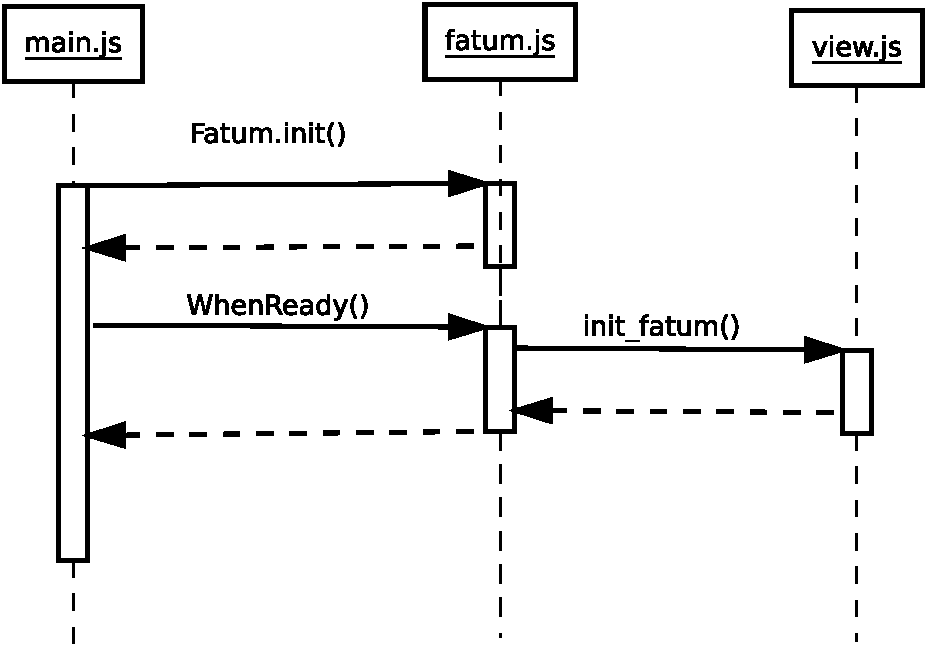
\includegraphics[width=0.75\textwidth]{diagram/document.pdf}
        \caption{Chargement de la page}
        \label{fig:chargement}
\end{figure}
Quand l'URL est saisi, la page se met à charger sans aucune intervention de l'utilisateur.
La figure \ref{fig:chargement} représente les différents appels de fonctions lors du chargement de la page. En effet, le chargement se fait par l'initialisation de \textit{FATuM} appelé dans le fichier {\tt view.js} qui appelle la bibliothèque {\tt fatum.js}.

\subsection{Lancement de la simulation}
Lorsque le bouton {\it Run} est cliqué, une série d'actions se produit.
D'abord, le cluster est affiché (sans les connections). Ensuite, le traitement de {\it MapReduce} est effectué. Enfin, les connections entre les slots sont affichées.\\
Ces actions sont représentées par trois parties dans les figures \ref{fig:run}, \ref{fig:ProMapRed} et \ref{fig:connection}.
\begin{figure}[H]
  \centering
    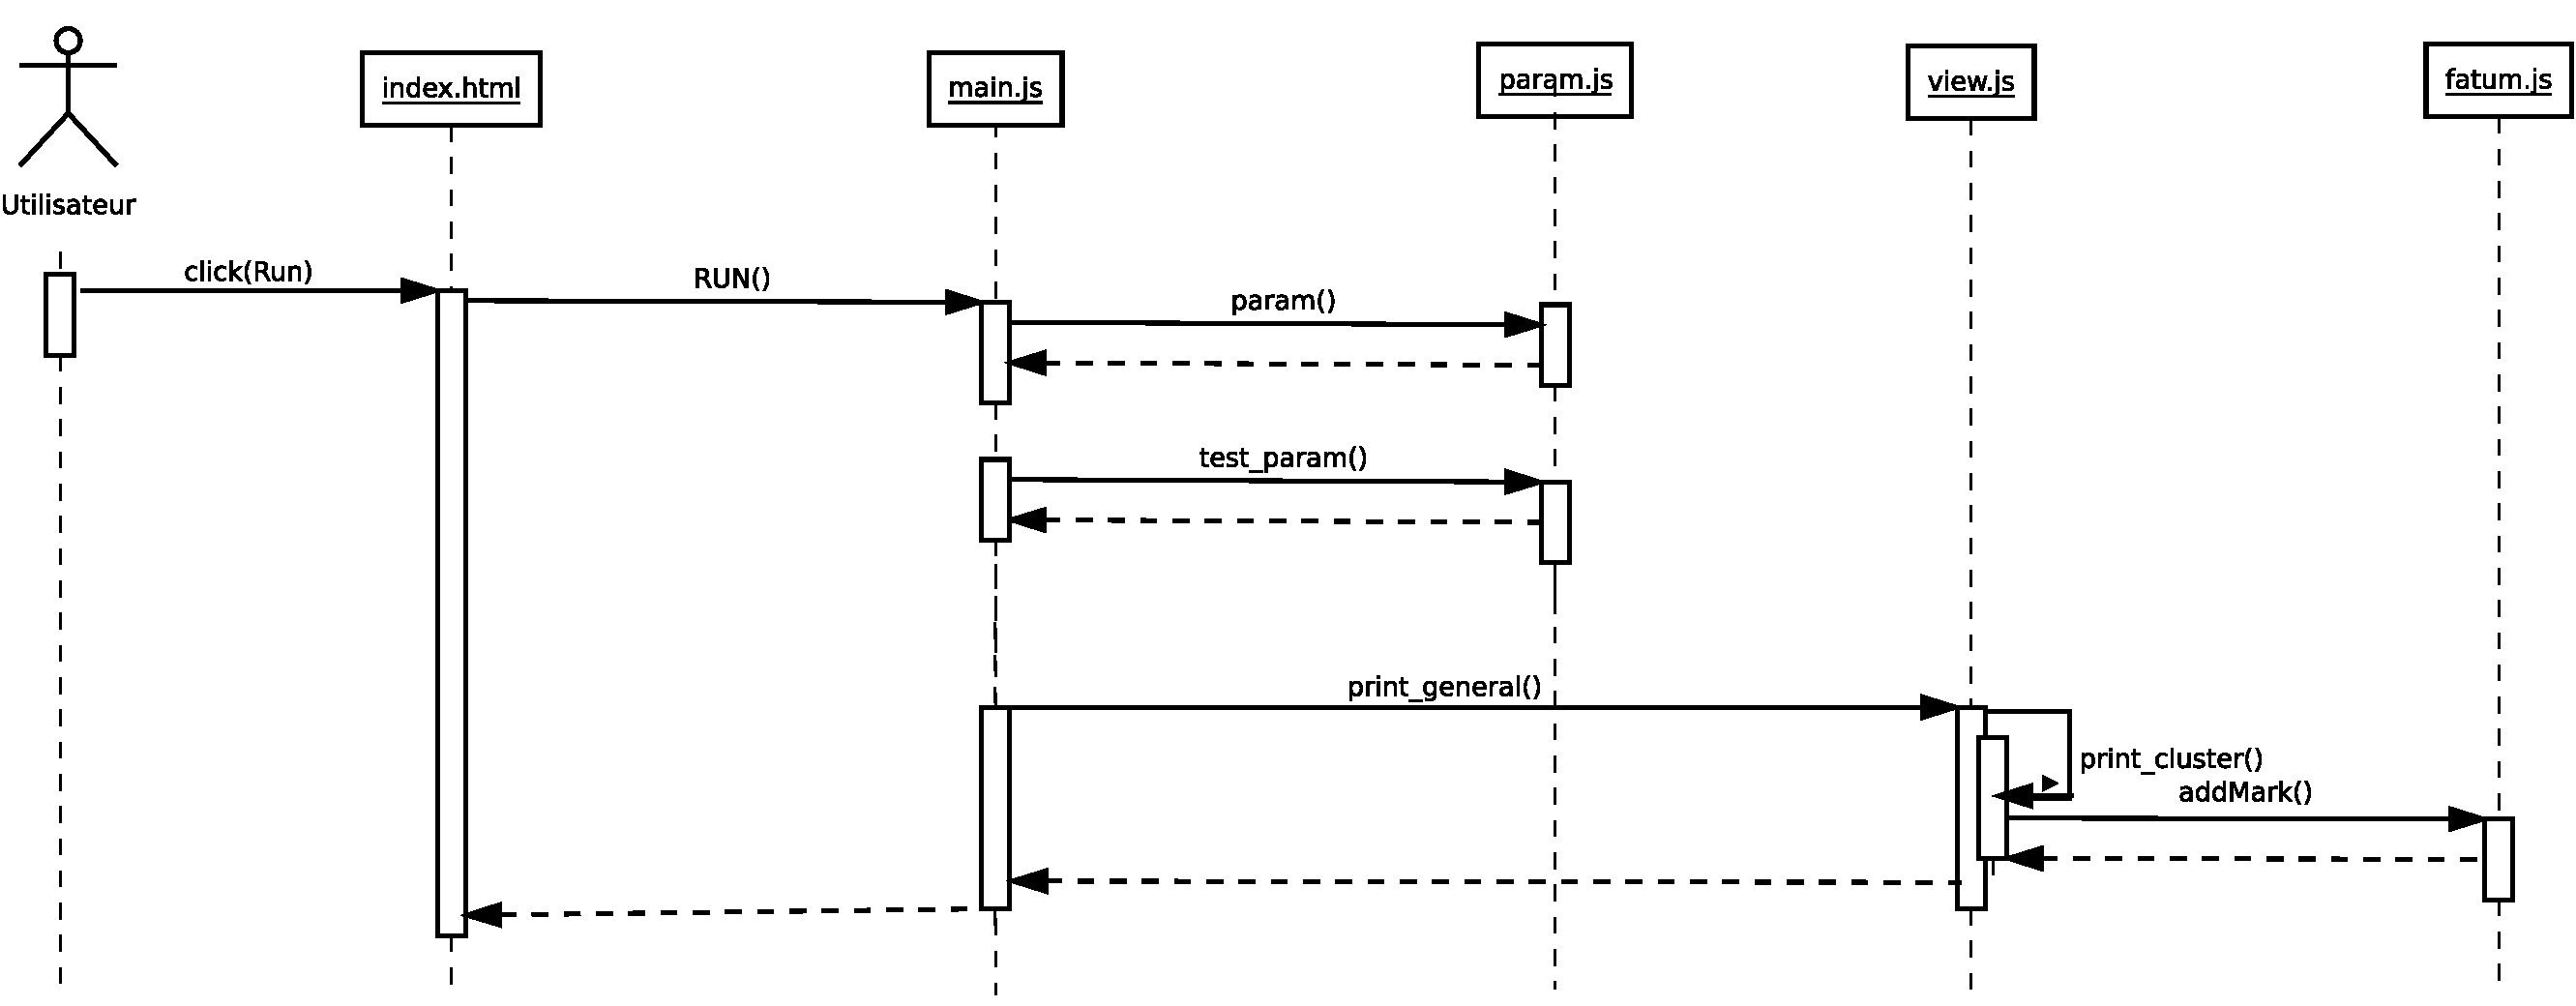
\includegraphics[angle=90,height=0.95\textheight]{diagram/diag_seq_init.pdf}
        \caption{Lancement du bouton RUN}
        \label{fig:run}
\end{figure}

\begin{figure}[H]
  \centering
    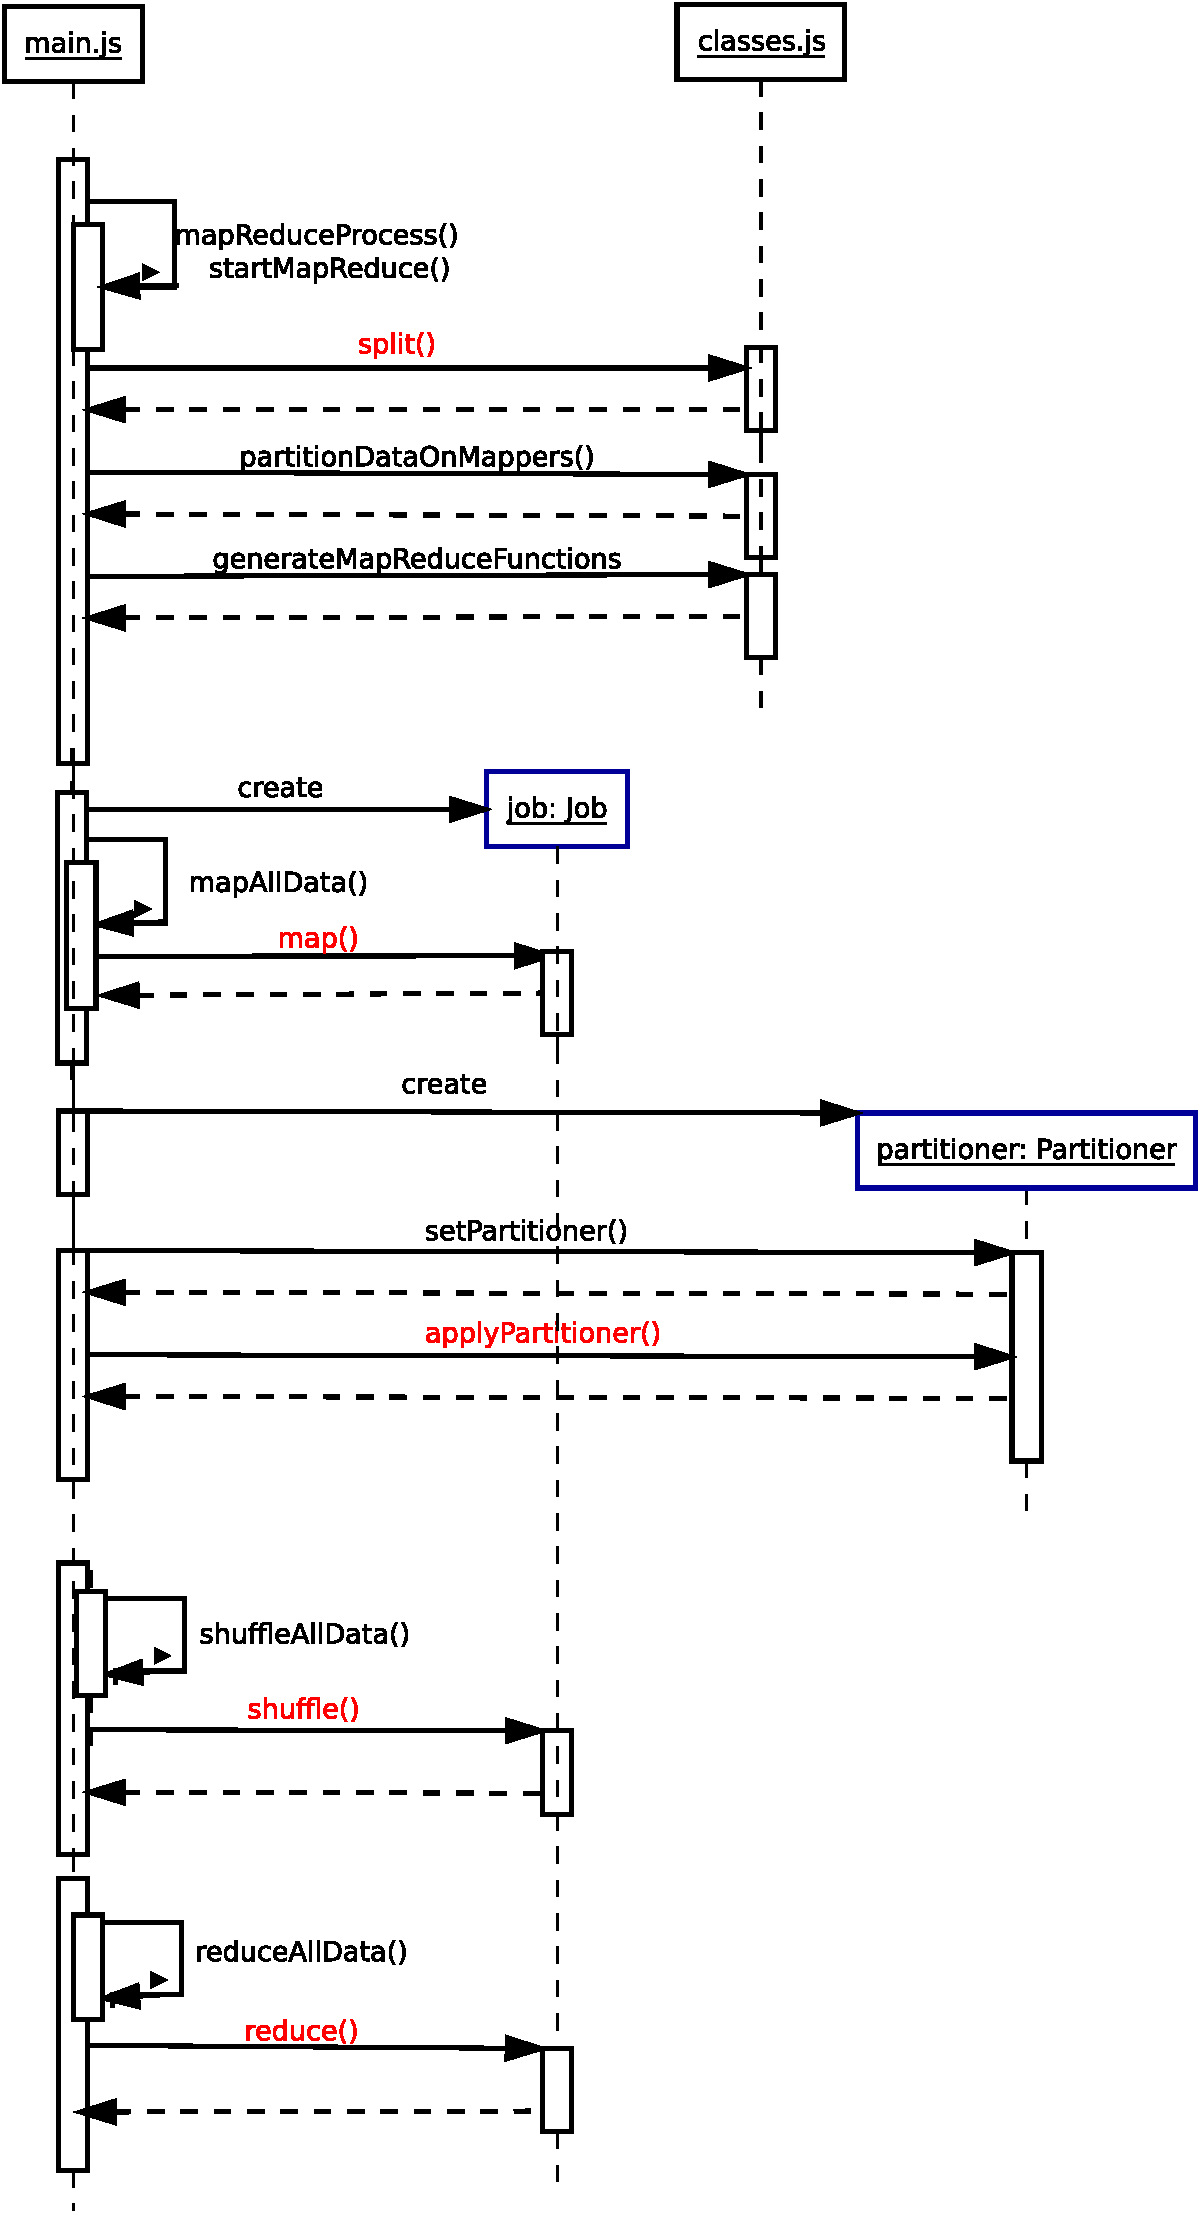
\includegraphics[height=0.95\textheight]{diagram/diag_seq_mapReduce.pdf}
        \caption{Process de MapReduce}
        \label{fig:ProMapRed}
\end{figure}

Lors de l'affichage du cluster, les données fournies par l'utilisateur doivent respecter certaines conditions imposées par la fonction {\tt Test\_param} (par exemple entrer un nombre supérieur à 1 pour le nombre de PC). Une fois les conditions d'utilisation passées, on appelle la bibliothèque {\it FATuM} pour afficher les différents slots du cluster de {\tt map()} et de {\tt reduce()} ainsi que les numéros des machines (affichage sans les connections entre les slots).

Une fois les éléments du cluster de la simulation affichés, le traitement des données s'effectue. Après chaque traitement, on effectue un lien entre chaque slot du cluster pour indiquer le transfert des données au sein de ce dernier représenté par des flèches provenant de {\it FATuM}.

\begin{figure}[H]
  \centering
    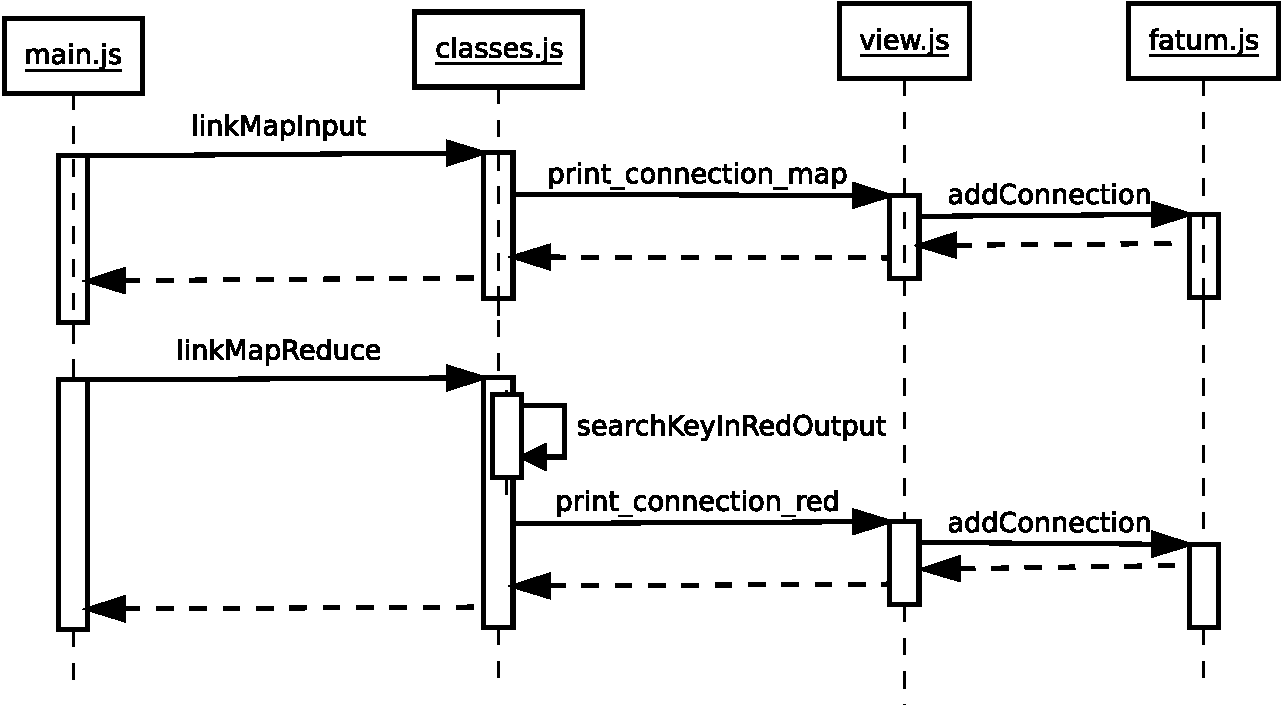
\includegraphics[width=0.75\textwidth]{diagram/print_connection.pdf}
        \caption{Affichage des connections}
        \label{fig:connection}
\end{figure}

\subsubsection{Téléchargement des résultats}
\begin{figure}[H]
  \centering
    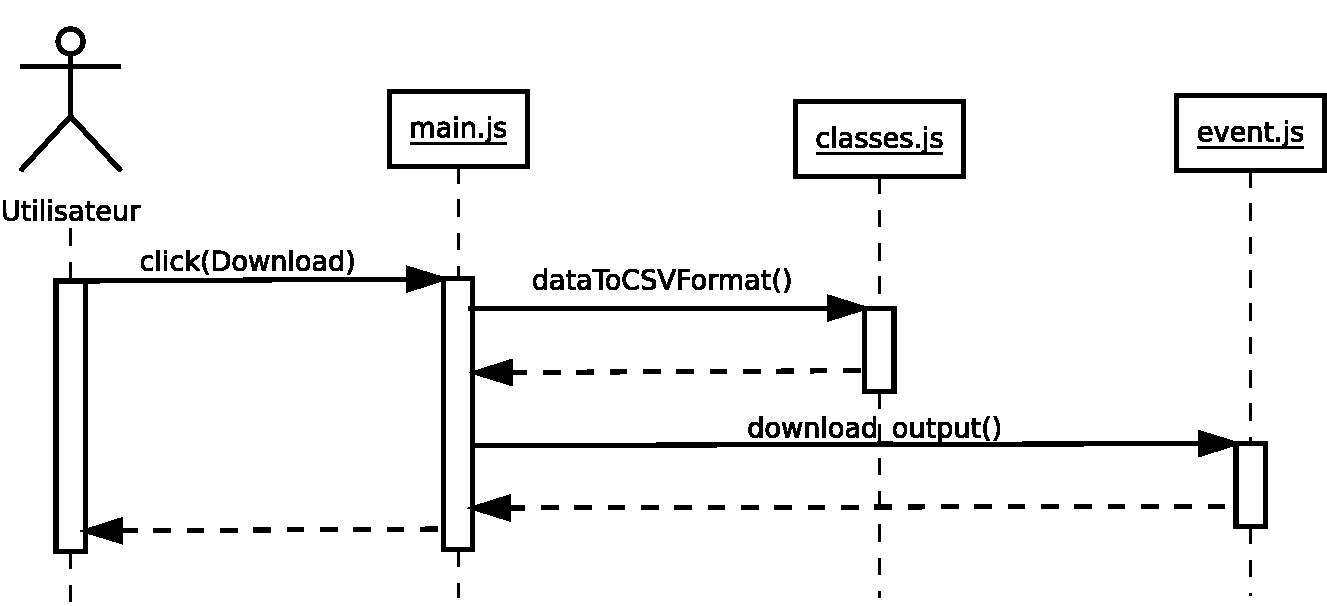
\includegraphics[width=0.75\textwidth]{diagram/download.pdf}
        \caption{Lancement du bouton Download}
        \label{fig:DL}
\end{figure}

Une fois la simulation et le traitement des données effectué. L'utilisateur peut récupérer ces données transformer par ses fonctions {\it MapReduce} en les téléchargeant dans un format {\tt .csv} (Figure \ref{fig:DL}).

\section{Partie graphique}


\subsection{Coté interface utilisateur}
\subsubsection{MaterializeCSS}
Pour l'interface utilisateur, nous avons dû utiliser la bibliothèque graphique \href{http://www.materializecss.com/}{{\tt MaterializeCSS}} qui fournit un dossier compressé comprenant tous les fichiers de base d'un site web. Ceci permet d'avoir une architecture de fichiers déjà existante et fournir les fichiers CSS nécessaires pour avoir un visuel optimisé et un design attirant.

Ainsi, il suffit d'appeler un élément graphique de HTML, de lui donner la classe correspondante implémentée dans MaterializeCSS et le visuel est prêt.

%%
\subsubsection{Structure du site}

Le site est en {\tt monopage}, c'est à dire qu'il n'y a pas de présence de plusieurs fichiers HTML à charger ou d'un serveur avec une base de données pour les différents élements.

Pour passer d'un contenu à un autre, nous utilisons l'élément HTML de "navigation". Ainsi, cela donne l'effet de trois pages: "Acceuil", "Commencer" et "A Propos" alors qu'il ne s'agit que d'un seul fichier HTML.\\

Dans la partie "Commencer", nous pouvons séparer cette partie en trois sous-catégories. La première permet à l'utilisateur de saisir ces paramètres (les fichiers de données, ses fonctions map/reduce et les paramètres du cluster).
La seconde permet soit d'écrire les fonctions map/reduce directement sur le site, ou de visualiser le code fournis pour le corriger directement.
Enfin la dernière section concerne la simulation avec FATuM pour le cluster et une colonne à droite de la page pour l'affichage des données contenues dans un slot.

\subsubsection{Les Loaders}
\begin{figure}[H]
  \centering
    
\includegraphics[scale=0.5]{images/loader.png}
        \caption{Loader}
\end{figure}
Le temps de chargement du site au démarrage ainsi que lors du lancement de la simulation sont long. Cette lenteur peut être interpréter comme un mauvais chargement des données par l'utilisateur. C'est pourquoi notre objectif était de rajouter un "loader" (voir Figure 4.1) au démarrage de la page pour signifier le chargement de FATuM et un autre pour le temps de calcul de la simulation. Le loader du démarrage fonctionne, malheureusement, celui de la simulation n'a pas pu être implémenter. En effet, le site se bloque le temps de calcul ce qui empêche l'utilisation du loader.

\subsubsection{Les paramètres}
Les {\tt paramètres} données par l'utilisateur doivent remplir certaines conditions.
\begin{itemize}
\item Le cluster du Map doit au grand maximum contenir entre 1 et 20 pc et entre 1 et 24 coeur . \\ Cette limitation est visuelle car au delà, la lisibilité n'est plus assuré. Il s'agit là, d'un choix suite aux conseils du client.
\item Le cluster de Reduce doit être comprise entre 1 et le nombre de slots total du cluster de Map.
\item Le fichier js des fonctions map/reduce n'étant pas nécessaire pour l'utilisation car nous avons fournit un exemple de code dans "section  code" qui est utilisé pour la suite de l'application.
\item Le fichier csv doit être impérativement fournit et contenir des données.
Si l'utilisateur rafraîchit la page, cette variable disparaît, il faut donc la charger de nouveau.
\end{itemize}


\subsection{Simulation graphique(Fatum)}
Comme demandé par le client, nous avons utilisé la bibliothèque graphique \href{http://www.labri.fr/perso/aperrot/fatum/index.html}{{\tt FATuM}} développée au \href{http://www.labri.fr/}{{\tt LABRI}}. Cette bibliothèque permet d'afficher la simulation du cluster (voir Figure 4.2) avec différents composants graphiques et ne peut être utiliser pour l'interface utilisateur contrairement à MaterializeCSS.
%image fatum simple avec connection.
\begin{figure}[H]
  \centering
    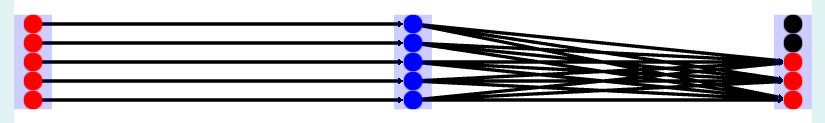
\includegraphics[scale=0.5]{images/graphiqueExemple.png}
        \caption{FATuM - Simulation}
\end{figure}

Nous utilisons plusieurs composants de FATuM:
\begin{itemize}
\item Les Marks
\item Les Connections
\item Le zoom
\item Une partie de la gestion d'un "clic souris"\\
\end{itemize}

\begin{figure}[H]
  \centering
    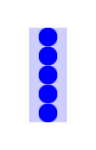
\includegraphics[scale=0.5]{images/marks.png}
        \caption{FATuM : Marks}
\end{figure}
Un {\tt Mark} (comme dans la figure ci-dessus) est un élément sous forme de cercle qui représente un slot du cluster. Ils sont séparés entre eux lorsque la limite de slots par PC est atteinte. Ainsi, chaque PC sont séparés graphiquement. Ces éléments graphiques sont dépendants des données fournies par l'utilisateur.\\

Les {\tt connections} sont les flèches qui vont d'un Mark vers un autre. Ils représentent le transfert de données entre les slots. On trouve des connections entre l'input de map et map ainsi que des connections entre map et reduce.\\

Le {\tt zoom} permet (si l'on pose le pointeur de la souris dans la zone de simulation gérée par FATuM) la gestion de la molette de la souris. Ainsi, en cas d'un gros cluster, l'ensemble reste lisible grâce à ce zoom. \\

Enfin, la gestion du {\tt "clic souris"}. Lors d'un clic dans la zone de simulation FATuM, les coordonnées récupérées sont celles de la fenêtre. Elles n'ont donc rien à voir avec celles de FATuM. La fonction {\tt windowToModel} nous a permis de transformer les coordonnées du clic en coordonnées compréhensibles par FATuM pour pouvoir exécuter le traitement suivant la zone de clic.


\subsubsection{Précision sur la fonction "search\_mark"}

\begin{lstlisting}
function search_mark(x, id) {
    var header_data, tmp_header;
    //type of the mark
    switch (x) {
        case indice_fatum_1:
            tmp_header = "Map Input--";
            break;

        case indice_fatum_2:
            tmp_header = "Map Output--";
            break;

        case indice_fatum_3:
            tmp_header = "Reduce Output--";
            break;
        default:
            return false;
    }
    var min = nb_slot + gap;
    var max = min + nb_slot;
    //researh the true id without the gap
    for (var i = 0; i < nb_pc; i++) {
        if (0 <= id && id < nb_slot) {
            header_data = "Slot " + id + ": --"; //exple: Slot 1: --Map Task--
            print_data(x, id, header_data + tmp_header);
            break;
        } else
        if (min <= id) {
            if (id < max) {
                id = id - (gap * (i + 1));
                header_data = "Slot " + id + ": --";
                print_data(x, id, header_data + tmp_header);
                break;
            }
        }
        min = max + gap;
        max = min + nb_slot;
    }
}
\end{lstlisting}

Cette fonction est particulière nécessite des précisions. 

En effet, pour différencier les blocs de pc, nous avons décider de mettre un décalage (variable gap) entre ces blocs. Ce décalage créer des erreurs d'id de mark par la suite. En effet, lorsque l'on clique sur un slot, sont id correspond à sa position dans l'axe y. Mais a cause de ce décalage, l'espacement était également considérer comme un bloc et les id était décaler.\\

D'autre part, cette fonction permet également de détecter quelle type de donnée on souhaite afficher. Pour cela, on utilise l'axe des x pour se repérer.

\subsubsection{La sortie console}

\begin{figure}[H]
  \centering
    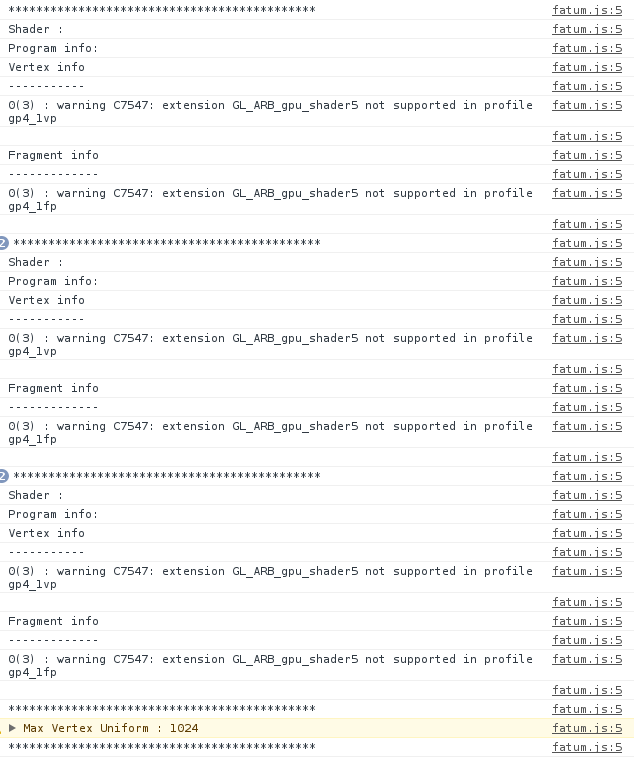
\includegraphics[scale=0.5]{images/console_fatum.png}
        \caption{Sortie console au démarrage}
\end{figure}
Lors du démarrage de l'application, l'initialisation de FATuM se fait, il est donc normal de voir en console (voir Figure 4.4), des informations concernant la bibliothèque.

\subsection{Difficulté lié à l'affichage}
Nos difficultés se sont principalement portées du fait que nous étions des débutants en web. Ainsi lorsqu'il a fallu utiliser la bibliothèque FATuM, les documentations n'étaient pas évidentes à comprendre au début. Surtout du fait que nous avions des exemples d'implémentation de FATuM dans une ancienne version de la documentation qui nous était fort utile pour comprendre les fonctions mais qui n'existaient plus pour certaines dans la nouvelle implémentation de FATuM.\\ 

Dans la nouvelle version de la documentation, il n'y a que les énoncés des fonctions, et c'est avec le temps que nous avons pris l'habitude de voir les exemples d'implémentation de FATuM dans l'ancienne documentation puis nous référer à la nouvelle documentation pour voir ce qui a changé.\\

\subsection{Amélioration possible}
Plusieur éléments peuvent être rajouté à la partie graphique pour améliorer l'utilisation de l'utilisateur et que nous n'avons pas pu implémenter
\begin{itemize}
\item le scrolling horizontal des données
\item un loader pour la simulation
\item Une optimisation visuelle du cluster
\end{itemize}


\paragraph{}
Concernant la partie visualisation, nous avons pensé que, plutôt que de rendre le cluster linéaire, c'est à dire: entrée Map puis sortie Map puis sortie Reduce chacun en ligne, le rendre cyclique.

\begin{figure}[H]
  \centering
    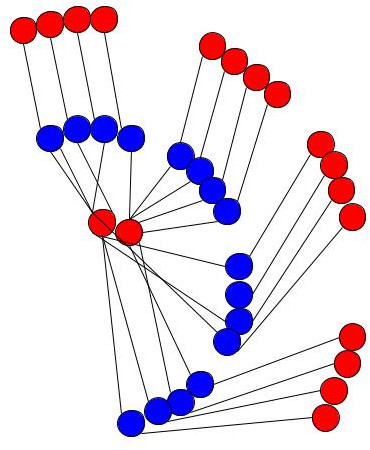
\includegraphics[scale=0.5]{images/cyclique.jpg}
        \caption{Exemple d'affichage}
\end{figure}
Ainsi, un très gros cluster serait plus ludique et plus compréhensible mais pourrait créer deux problèmes: il n'y a plus la linéarité du map reduce comme indiqué dans la littérature et les connections de fatum sont moins lisibles car elles vont traversé les marks intérieur.\\

Enfin, il y existe un conflit avec webGL. Nous ignorons à quoi ce bug est dû mais, il arrive que le navigateur ait des soucis avec cette bibliothèque. Ce problème peut être lié au cache. Mais nous n'avons pas de solution à proposer

\newpage
\section{Partie interpréteur}



\subsection{Les classes}

En Javascript, l'implémentation des classes peut se faire de plusieurs manières. Il existe la façon avec le mot clé '{\tt class}'. Cette manière, bien que plus claire et plus facile à comprendre, n'est pas supportée par tous les navigateurs. Et comme la portabilité est l'un de nos besoins de qualité, nous avons préféré la manière "classique" de créer des classes en Javascript.

La déclaration est par contre un peu différente des autres langages Orientés Objet comme Java ou C++. Nous donnons l'exemple suivant de l'implémentation de la classe {\tt Job}:\\

\begin{lstlisting}

function Job(map, reduce) { 
    this.map = map;
    this.reduce = reduce;
}

Job.prototype.applyMap = function(data) {
	... //Appel a this.map 
}

Job.prototype.applyReduce = function(data) {
    ... //Appel a this.reduce
}

\end{lstlisting}

%En plus de cette classe, nous utilisons 

\subsection{Retranscription du process mapReduce}


Pour les besoins de notre projet, nous n'avons pas basé notre implémentation du code sur les classes mais plutot sur les fonctions. Pour cela, nous avons centré le code de l'interpréteur dans un seul fichier .js qui contient, en plus des classes du projet, les fonctions qui interprétent le code mapReduce pour fournir les sorties (outputs).

\subsubsection{Fonction split}

\subsubsection{Fonction eval}

\subsubsection{Fonction partitionDataOnMappers}



\subsection{Les expressions régulières}

L'un des problèmes qui peuvent s'imposer est que le retour à la ligne n'est pas le même sous les différents systèmes d'exploitation (Linux, Windows et macOS). En effet, sous Windows le retour à la ligne est décelé avec "\escape{n}" alors que sous MacOS c'est fait avec "\r". 	
Nous avons donc utilisé une expression régulière dans la fonction {\tt split()} pour séparer les lignes du fichier {\tt CSV} quelque soit le système d'exploitation sous lequel il a été écrit.\\

Dans la même fonction split, on utilise une autre expression régulière 
%%ici apparait Big Data


\subsection{Difficultés rencontrées}

- Apprentissage du process de mapReduce (a pris du temps etc)\\
- Retranscrire la distribution normalement faite par Hadoop.\\
- Récupérer les fonctions en JS écrites par l'utilisateur et les appliquer sur les données.

\subsection{Limitations}
- Pas de free pour les tasks terminées.\\
- Malheureusement, pour des contraintes de temps, nous n'avons pas réussi à implémenter la phase de combiner ni l'exportation du code mapReduce en Java.\\
- Gestion d'erreurs: 

{\bf Amélioration possible:} rajouter un analyseur syntaxique pour le code javascript entré et faire un retour à l'utilisateur sur les erreurs potentiellement commises sur son code.

\section{Limitations}

\subsection{Difficultés rencontrées}
{\bf FATuM}\\

Etant des débutants en programmation Web, il nous a fallu du temps pour comprendre comment utiliser la bibliothèque {\it FATuM}. C'est grâce aux documentations que nous nous sommes familiarisés avec la bibliothèque même si elles n'étaient pas évidentes à comprendre au début. Une ancienne version de la documentation nous a été fortement utile pour comprendre les fonctions fournies par la bibliothèque (même si certaines fonctions n'existent plus dans l'implémentation de {\it FATuM} la plus récente).\\ 

Dans la nouvelle version de la documentation, il n'y a que les énoncés des fonctions, et c'est avec le temps que nous avons pris l'habitude de voir les exemples d'implémentation de {\it FATuM} dans l'ancienne documentation puis nous référer à la nouvelle documentation pour voir ce qui a changé.\\

{\bf MapReduce}\\
\begin{itemize}
\item L'une des étapes de réalisation du projet qui a demandé le plus d'effort est la compréhension du fonctionnement de {\it MapReduce}. En effet, nous avons senti l'importance de bien comprendre comment l'exécution se fait puisque notre projet revient à retranscrire l'exécution sans un framework pour {\it MapReduce}.\\
Cela a représenté un réel défi de retranscrire la distribution normalement faite par Hadoop.\\

\item Récupérer les fonctions écrites en Javascript par l'utilisateur et les appliquer sur les données.\\

\item Redéfinir la fonction de hashage puisqu'elle est implémenté en langage Java mais n'existe pas en Javascript. 
\end{itemize}

\subsection{Amélioration possible}
{\bf FATuM}\\
Plusieur éléments peuvent être rajoutés à la partie graphique pour améliorer l'utilisation de l'application. Nous citons quelques uns:\\
\begin{itemize}
\item Le scrolling horizontal des données.
\item Un loader pour la simulation.
\item Une optimisation visuelle du cluster.
\end{itemize}

\paragraph{}
Il existe un conflit avec {\it WebGL} qui peut, dans des cas exceptionnels, causer la non-initialisation de {\it FATuM}. Nous ignorons à quoi ce bogue est dû, mais il arrive que le navigateur aie des soucis avec cet élément. Ce problème peut être lié au cache. Mais nous n'avons pas de solution à proposer.

Concernant la partie visualisation, nous avons pensé à rendre cyclique l'affichage des éléments de la simulation(c'est-à-dire: entrée {\tt map()} puis sortie {\tt map()} puis sortie {\tt reduce()} chacun en une colonne). Nous montrons l'affichage tel que nous l'avons imaginé dans la figure \ref{fig:possibilite}.

\begin{figure}[H]
  \centering
    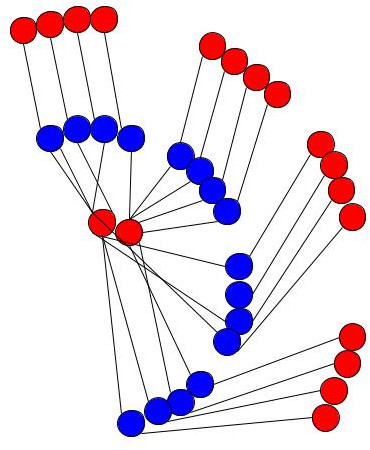
\includegraphics[width=0.5\textwidth]{images/cyclique.jpg}
        \caption{Affichage cyclique de la simulation}
        \label{fig:possibilite}
\end{figure}
Ainsi, un très gros cluster serait plus lisible que la version d'affichage actuelle. Mais dans ce cas, elle peut créer deux soucis: il n'y a plus la linéarité du {\it MapReduce} comme attendu et les connections de {\it FATuM} sont moins lisibles car elles vont traverser les marks qui sont à l'intérieur.\\

{\bf MapReduce}\\

L'une des améliorations possibles est de libérer de l'espace mémoire à chaque fois qu'une tâche a terminé son exécution. Ceci peut donc servir dans le cas d'un très grand fichier de données.\\

Malheureusement, pour des contraintes de temps, nous n'avons pas réussi à implémenter la phase de {\it combiner} ni l'exportation du code {\it MapReduce} en Java qui auraient complété l'implémentation de {\it MapReduce}.\\

Nous pouvons aussi rajouter la gestion d'erreurs :
Ajouter un analyseur syntaxique pour le code Javascript entré et faire un retour à l'utilisateur sur les erreurs potentiellement commises sur son code.

\section{Indentation du code}

L'indentation du code est garantie par l'outil {\tt js-beautify}\footnote{\url{https://github.com/beautify-web/js-beautify}}
qui uniformise la forme du code javascript que nous avons réalisé. Cela permet de traiter automatiquement une partie de la factorisation du code.

L'utilisation de règles de codage permet de faciliter la lecture du code source produit entre les développeurs et de minimiser la complexité du code qui peux mener sur le long terme à l'introduction de bogues dans le logiciel.

\subsection{Exemple du résultat produit par {\tt js-beautify}}
Le code est donné à titre d'exemple uniquement et ne fais pas parti du code source de notre projet.

\begin{figure}[H]
\begin{lstlisting}
Partitioner.prototype.apply = function(foo, bar) {
  var a=[],tmp;
  var z,y,x,w;

  for(var i=0;i<foo.len;i++){
    y=foo[i];
    z=this.get(y.key,y.val,bar);

    w=false;
    x=0;
    if(a.len==0){
      tmp=[];
      tmp.push(y);
      a.push(tmp);}
    else{
      while(!w && x<a.len){
        if(z==this.get(a[x][0].key,a[x][0].val,bar)){
          w=true;
          a[x].push(y);}
        x++;}
        if(!w){
          tmp=[];
          tmp.push(y);
          a.push(tmp);}}}
  return a;}
\end{lstlisting}
\caption{Code avant passage de {\tt js-beautify}}
\end{figure}

\begin{figure}[H]
\begin{lstlisting}
Partitioner.prototype.apply = function(foo, bar) {
    var a = [],
        tmp;
    var z, y, x, w;

    for (var i = 0; i < foo.len; i++) {
        y = foo[i];
        z = this.get(y.key, y.val, bar);

        w = false;
        x = 0;
        if (a.len == 0) {
            tmp = [];
            tmp.push(y);
            a.push(tmp);
        } else {
            while (!w && x < a.len) {
                if (z == this.get(a[x][0].key, a[x][0].val, bar)) {
                    w = true;
                    a[x].push(y);
                }
                x++;
            }
            if (!w) {
                tmp = [];
                tmp.push(y);
                a.push(tmp);
            }
        }
    }
    return a;
}
\end{lstlisting}
\caption{Code après passage de {\tt js-beautify}}
\end{figure}
